\documentclass[border=2pt]{standalone}
\usepackage[T1]{fontenc}
\usepackage[tt=false]{libertine}
\usepackage[libertine]{newtxmath}
\usepackage{xcolor}
\usepackage{tikz}
\usetikzlibrary{arrows.meta}
\definecolor{archCNN}{HTML}{2A78D6}
\definecolor{archTR}{HTML}{1BAF7A}
\definecolor{archHY}{HTML}{EB6834}
\definecolor{archGrey}{HTML}{6B6B6B}
\definecolor{archPU}{HTML}{5B4FA8}
\definecolor{archOK}{HTML}{2F7A3C}
\begin{document}
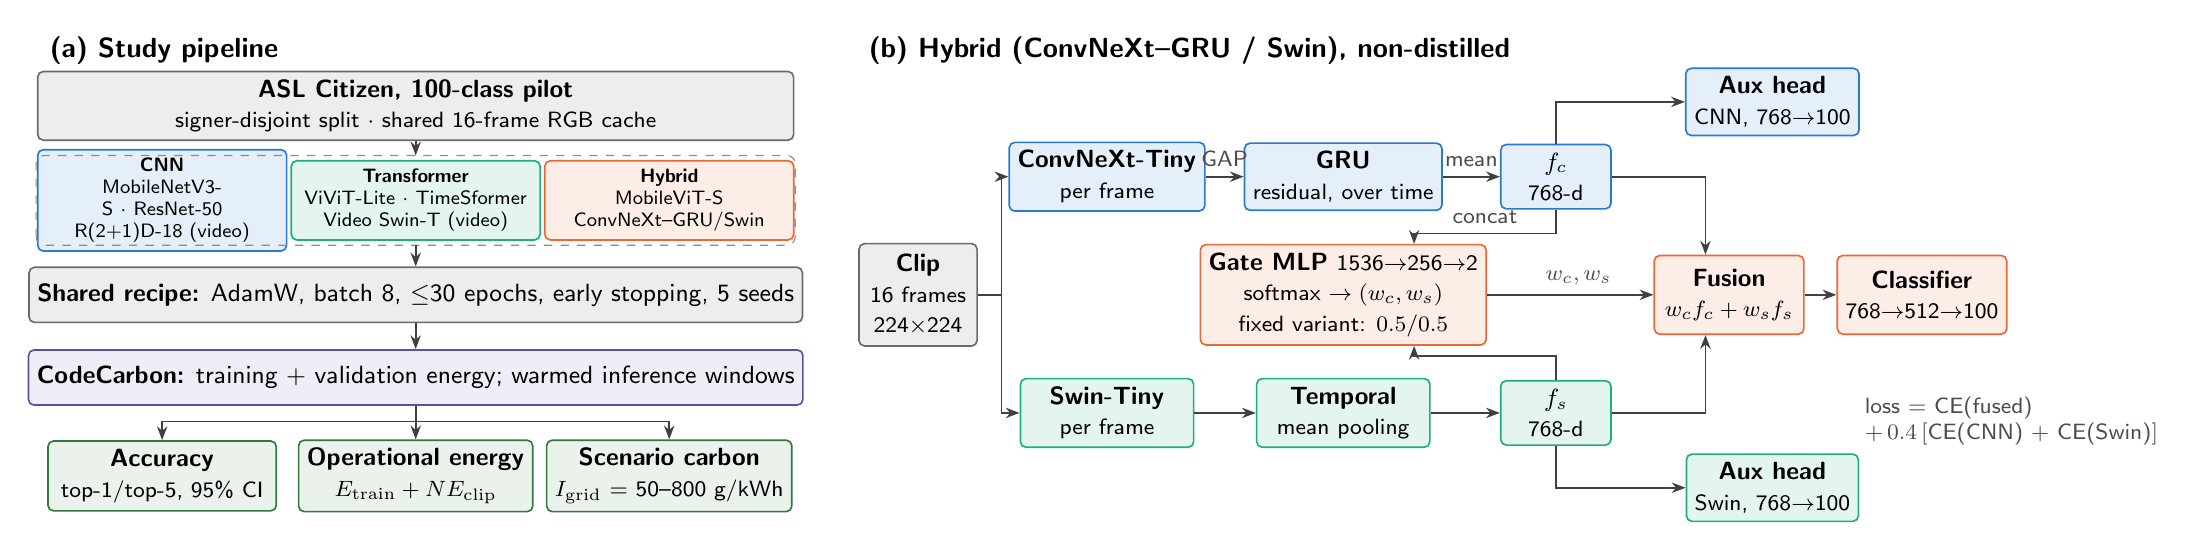
\begin{tikzpicture}[
      font=\sffamily\small,
      box/.style={draw, rounded corners=2pt, line width=0.6pt, align=center, inner sep=3pt},
      gbox/.style={box, fill=archGrey!12, draw=archGrey},
      cbox/.style={box, fill=archCNN!12, draw=archCNN},
      tbox/.style={box, fill=archTR!12, draw=archTR},
      hbox/.style={box, fill=archHY!12, draw=archHY},
      pbox/.style={box, fill=archPU!10, draw=archPU},
      obox/.style={box, fill=archOK!10, draw=archOK},
      fbox/.style={minimum width=3.05cm, text width=2.95cm, minimum height=1.0cm, font=\sffamily\scriptsize},
      arr/.style={-{Stealth[length=5pt]}, line width=0.6pt, draw=black!75},
      lab/.style={font=\sffamily\footnotesize, text=black!70}
    ]
    %% ---------------- (a) study pipeline ----------------
    \node[font=\sffamily\bfseries, anchor=west] at (0.0,6.15) {(a) Study pipeline};
    \node[gbox, minimum width=9.6cm, minimum height=0.8cm] (data) at (4.77,5.45)
      {\textbf{ASL Citizen, 100-class pilot}\\ {\footnotesize signer-disjoint split $\cdot$ shared 16-frame RGB cache}};
    \node[cbox, fbox] at (1.55,4.25) {\textbf{CNN}\\ MobileNetV3-S $\cdot$ ResNet-50\\ R(2+1)D-18 (video)};
    \node[tbox, fbox] at (4.77,4.25) {\textbf{Transformer}\\ ViViT-Lite $\cdot$ TimeSformer\\ Video Swin-T (video)};
    \node[hbox, fbox] at (7.99,4.25) {\textbf{Hybrid}\\ MobileViT-S\\ ConvNeXt--GRU/Swin};
    \draw[dashed, draw=black!45, rounded corners=3pt] (-0.05,3.68) rectangle (9.59,4.82);
    \node[gbox, minimum width=9.6cm, minimum height=0.7cm] (rec) at (4.77,3.05)
      {\textbf{Shared recipe:} AdamW, batch 8, $\leq$30 epochs, early stopping, 5 seeds};
    \node[pbox, minimum width=9.6cm, minimum height=0.7cm] (cc) at (4.77,2.0)
      {\textbf{CodeCarbon:} training + validation energy; warmed inference windows};
    \node[obox, minimum width=2.9cm, minimum height=0.85cm] (o1) at (1.55,0.75) {\textbf{Accuracy}\\ {\footnotesize top-1/top-5, 95\% CI}};
    \node[obox, minimum width=2.9cm, minimum height=0.85cm] (o2) at (4.77,0.75) {\textbf{Operational energy}\\ {\footnotesize $E_{\mathrm{train}} + N E_{\mathrm{clip}}$}};
    \node[obox, minimum width=2.9cm, minimum height=0.85cm] (o3) at (7.99,0.75) {\textbf{Scenario carbon}\\ {\footnotesize $I_{\mathrm{grid}}$ = 50--800 g/kWh}};
    \draw[arr] (data.south) -- (4.77,4.82);
    \draw[arr] (4.77,3.68) -- (rec.north);
    \draw[arr] (rec.south) -- (cc.north);
    \draw[line width=0.6pt, draw=black!75] (cc.south) -- ++(0,-0.2) coordinate (s);
    \draw[arr] (s) -| (o1.north);
    \draw[arr] (s) -- (o2.north);
    \draw[arr] (s) -| (o3.north);

    %% ---------------- (b) hybrid architecture ----------------
    \node[font=\sffamily\bfseries, anchor=west] at (10.4,6.15) {(b) Hybrid (ConvNeXt--GRU / Swin), non-distilled};
    \node[gbox, minimum width=1.5cm, minimum height=1.3cm] (in) at (11.15,3.05) {\textbf{Clip}\\ {\footnotesize 16 frames}\\ {\footnotesize 224$\times$224}};
    % CNN branch
    \node[cbox, minimum width=2.2cm, minimum height=0.8cm] (cnx) at (13.55,4.55) {\textbf{ConvNeXt-Tiny}\\ {\footnotesize per frame}};
    \node[cbox, minimum width=2.2cm, minimum height=0.8cm] (gru) at (16.55,4.55) {\textbf{GRU}\\ {\footnotesize residual, over time}};
    \node[cbox, minimum width=1.4cm, minimum height=0.8cm] (fc) at (19.25,4.55) {$f_c$\\ {\footnotesize 768-d}};
    % Swin branch
    \node[tbox, minimum width=2.2cm, minimum height=0.8cm] (swin) at (13.55,1.55) {\textbf{Swin-Tiny}\\ {\footnotesize per frame}};
    \node[tbox, minimum width=2.2cm, minimum height=0.8cm] (tp) at (16.55,1.55) {\textbf{Temporal}\\ {\footnotesize mean pooling}};
    \node[tbox, minimum width=1.4cm, minimum height=0.8cm] (fs) at (19.25,1.55) {$f_s$\\ {\footnotesize 768-d}};
    % gate, fusion, classifier
    \node[hbox, minimum width=2.9cm, minimum height=1.05cm] (gate) at (16.55,3.05) {\textbf{Gate MLP} {\footnotesize 1536$\to$256$\to$2}\\ {\footnotesize softmax $\to (w_c, w_s)$}\\ {\footnotesize fixed variant: $0.5/0.5$}};
    \node[hbox, minimum width=1.9cm, minimum height=1.0cm] (fuse) at (21.45,3.05) {\textbf{Fusion}\\ {\footnotesize $w_c f_c + w_s f_s$}};
    \node[hbox, minimum width=1.9cm, minimum height=1.0cm] (cls) at (23.9,3.05) {\textbf{Classifier}\\ {\footnotesize 768$\to$512$\to$100}};
    \node[cbox, minimum width=1.9cm, minimum height=0.8cm] (auxc) at (22.0,5.5) {\textbf{Aux head}\\ {\footnotesize CNN, 768$\to$100}};
    \node[tbox, minimum width=1.9cm, minimum height=0.8cm] (auxs) at (22.0,0.6) {\textbf{Aux head}\\ {\footnotesize Swin, 768$\to$100}};
    % arrows
    \draw[arr] (in.east) -- ++(0.3,0) |- (cnx.west);
    \draw[arr] (in.east) -- ++(0.3,0) |- (swin.west);
    \draw[arr] (cnx.east) -- node[lab, above] {GAP} (gru.west);
    \draw[arr] (gru.east) -- node[lab, above] {mean} (fc.west);
    \draw[arr] (swin.east) -- (tp.west);
    \draw[arr] (tp.east) -- (fs.west);
    \draw[arr] (fc.south) -- ++(0,-0.3) -| node[lab, pos=0.25, above] {concat} ([xshift=0.9cm]gate.north);
    \draw[arr] (fs.north) -- ++(0,0.3) -| ([xshift=0.9cm]gate.south);
    \draw[arr] (gate.east) -- node[lab, above, pos=0.55] {$w_c, w_s$} (fuse.west);
    \draw[arr] (fc.east) -| ([xshift=-0.3cm]fuse.north);
    \draw[arr] (fs.east) -| ([xshift=-0.3cm]fuse.south);
    \draw[arr] (fuse.east) -- (cls.west);
    \draw[arr] (fc.north) |- (auxc.west);
    \draw[arr] (fs.south) |- (auxs.west);
    \node[lab, align=left, anchor=west] at (23.05,1.45) {loss $=$ CE(fused)\\ $+\,0.4\,[$CE(CNN) $+$ CE(Swin)$]$};
  \end{tikzpicture}
\end{document}
